\section{System Description}
This project aims to make a system that will give the user the possibility to count a number of items by weighing items on a scale. 
The user will provide a known number of items, place the items on the scale and the Counting Scale system will calculate a scaling factor. 
There are a few default items already stored in the system with a scaling factor.
With this scaling factor, the user can place an unknown number of items on the scale, and the Counting Scale system will display the number of items placed on the scale. 
In \cref{fig:system} the structure of the Counting Scale system can be seen. \\

\noindent The Counting Scale system consists of the following parts:
\begin{itemize}
	\item Arduino ATMega2560
	\item ITDB02 TFT 240RGBx320 LCD
	\item ITDB02 LCD Shield
	\item Keypad
	\item Load cell
	\item Instrumentation Amplifier
\end{itemize}

\begin{figure}[H]
	\centering
	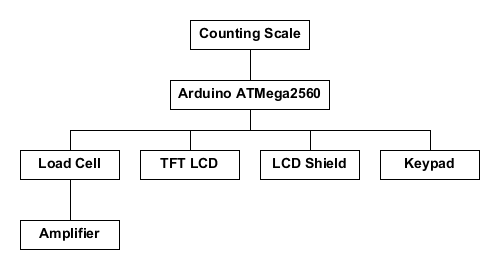
\includegraphics[width=0.6\linewidth]{graphics/system}
	\caption{Overall structure of the Counting Scale system.}
	\label{fig:system}
\end{figure}
\newpage

\noindent In \cref{fig:domainmodel} the associations between the conceptual classes of the Counting Scale system can be seen. 
The User presses a key on Keypad, the user interface, to start counting an item. 
The Arduino ATMega2560 scans the Keypad to detect if a key is pressed. 
The differential voltage from the Load Cell is gained by the Amplifier which gives a single ended output.
This signal is converted by the ADC of the Arduino ATMega2560.
The ADC output is converted to a weight and is scaled with a stored scaling factor for a given item to result in an amount of items placed on the scale.
The amount of items is displayed on the LCD.
\begin{figure}[H]
	\centering
	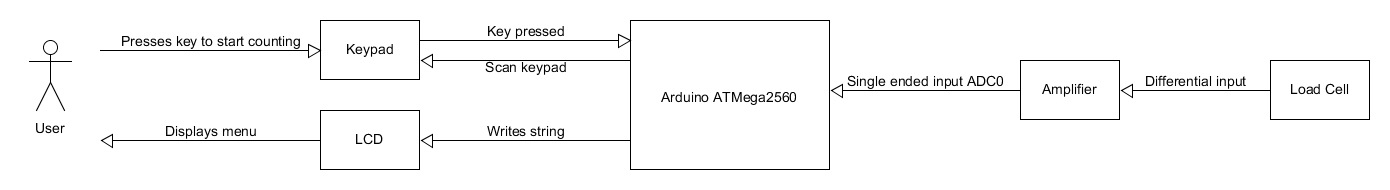
\includegraphics[width=\linewidth]{graphics/domainmodel}
	\caption{Domain Model of Counting Scale system functionality.}
	\label{fig:domainmodel}
\end{figure}